\documentclass[12pt]{article}

\usepackage{amsmath}    % need for subequations
\usepackage{graphicx}   % need for figures
\usepackage{verbatim}   % useful for program listings
\usepackage{color}      % use if color is used in text
\usepackage{subfigure}  % use for side-by-side figures
\usepackage{hyperref}   % use for hypertext links, including those to external documents and URLs

\author{P.~Gusev}
\title{NDN-RTC app design and protocol specification (DRAFT v0.1)}

\begin{document}

\maketitle
\newpage

%************************************************
\section*{Abstract}
\tableofcontents

\newpage
\section{Overview}
\subsection{Participants and institutions}
\begin{itemize}
\item Jeff Burke
\item Jeff Thompson
\item Peter Gusev
\item Qiuhan Ding
\end{itemize}

\subsection{Motivation}
The video conferencing tool is one of those apps which is needed first of all for internal use and experimenting with real-time communication over NDN. As we are interested in increasing NDN popularity among non-research peers as well, we are trying to provide easy-to-setup NDN apps by employing web browser APIs.

\subsection{Description}
NDN-RTC is a JavaScript application which utilizes the WebRTC engine for media encoding/decoding and C++ NDN library for the transport layer. The proposed initial app design contains two main modules: 
\begin{enumerate}
\item \textbf{Browser add-on} \\
Contains the NDN media-specific transport layer implementation, the encoding/decoding engine (WebRTC) and provides a JavaScript API for access from browser apps;
\item \textbf{JavaScript app} \\
Provides general conference discovery between peers
\end{enumerate}

The app borrows some ideas from previous work \cite{videoTR,ChronosTR}. It maintains synchronization of a digest tree in order to keep track of current chat participants in the same manner as ChronosChat \cite{ChronosTR}. Given that information, a new participant can start fetching media data objects from other peers (according to the media namespace presented on Figure \ref{media-ns}).

\begin{figure}
\centering
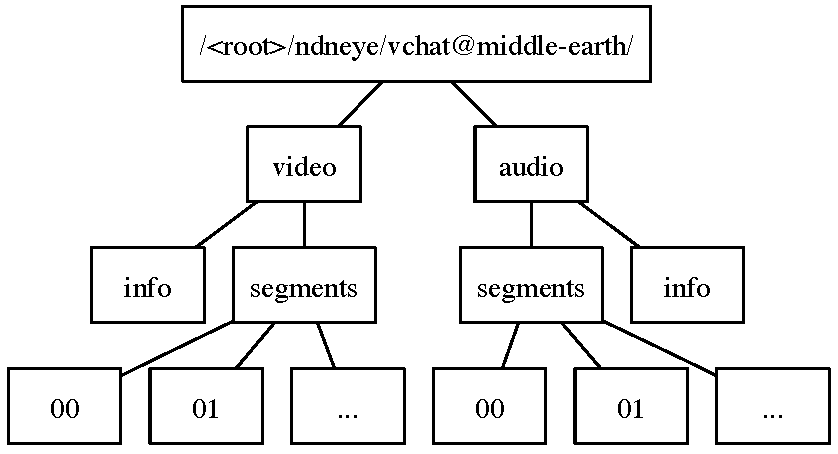
\includegraphics[width=0.8\textwidth]{../res/graphics/namespace-v01}
\caption{NDN-WebRTC Media Namespace}
\label{media-ns}
\end{figure}

The main goal of fetching media is to minimize the delay of receiving the latest frames. Having that in mind, we came up with the following design assumptions:

\begin{itemize}
\item Consumers are in full control of the speed of issuing media interests (i.e. interests in a segment namespace);
\item Most recent media frames are delivered by pipelining media interests at an a priori higher rate than the producer delivers them (since the peer can obtain framerate information from the other peer by questioning the "info" namespace, it can determine the frequency of interest issuing);
\item The presence of outstanding interests indicates retrieval of the most recent data;
\item If the consumer has no outstanding interests, she increases the interest rate or, depending on the average rendering time, switches to a lower media quality. 
\end{itemize} 

Since no synchronization problems need to be solved in such a "consumer" approach, we hope that NDN-WebRTC can show better results in scalability for many-to-many scenarios.

\section{Protocol specification}
\subsection{Discovery}
\textit{TBD}

\subsection{Real time communication}
\begin{enumerate}
\item Upon successful discovery of a video producer URI, the consumer issues an interest in the index namespace and gets data about the media stream's parameters ($FrameRate$ and codecs).
\item The consumer issues $Interest_{0}$ with the \textit{RigthMostChild=\textbf{true}} selector in the namespace for the frames like this: \textit{/root/mediadata} and waits until the first segment is received.
\item The consumer switches to \textbf{"Chase Mode"}
\end{enumerate}

\textbf{Chase Mode}
\begin{enumerate}
\item THe consumer extracts the frame number - $FN$ from the obtained $DataObject$ and pipelines interests at a rate of $2*FrameRate$ (twice the producer data rate) with \textit{RightMostChild=\textbf{true}} in the namespace for segments like this: \textit{/root/mediadata/FN/0}. i.e. the pipeline contains interests $Interest_{FN}$, $Interest_{FN+1}$, $Interest_{FN+2}$,...

\item The consumer watches two parameters: $DeliveryRate$ of frames, $RoundTripTime$ for interests:
\begin{itemize}
\item If $DeliveryRate$ is the same as $FrameRate$  and $RoundTripTime$ is not growing steadily, the consumer switches to \textbf{Fetch Mode} (see below)
\item If either $DeliveryRate$ and/or $FrameRate$ are growing, the consumer chooses a lower quality (by modifying the prefix) and re-enables \textbf{Chase Mode}
\end{itemize}
\end{enumerate}

\textbf{Fetch Mode}
\begin{enumerate}
\item The consumer extracts the latest frame number - $LFN$ and sets up a \textit{Frame interest} pipeline at a frequency of $2*FrameRate$:
\begin{center}
for a 24 fps video:
\begin{itemize}
\item \textbf{t = 0 sec} \\
Interest for \textit{/root/video/LFN/0}, timeout = 1.5 sec
\item \textbf{t = 1/48s} \\
Interest for \textit{/root/video/LFN+1/0}, timeout = 1.5 sec
\item \textbf{t = 2/48s} \\
Interest for \textit{/root/video/LFN+2/0}, timeout = 1.5 sec
\item ...
\end{itemize}
\end{center}

The number of segments per frame ($NumSegs$) is indicated using the \textit{FinalBlockID} field of each segment's DataObject. The consumer sets up a \textit{Segments interest} pipeline for each frame like this: 
\begin{center}
\begin{itemize}
\item Interest for \textit{/root/video/LFN/0}
\item Interest for \textit{/root/video/LFN/1}
\item Interest for \textit{/root/video/LFN/2}
\item ...
\item Interest for \textit{/root/video/LFN/$SegNum$}
\end{itemize}
\end{center}

\item The consumer periodically issues a \textbf{"probe"} interest with the last known frame number and \textit{RightMostChild=\textbf{true}} in order to detect a lag from the producer. If a considerable lag was detected, the consumer chooses stream parameters for a lower rate and switches to the \textbf{Chase Mode}

\item The consumer watches the value of $DeliveryRate$ and $RoundTripTime$ for the interests. If either of these values starts to grow, the consumer should choose stream parameters for a lower rate and switch to the \textbf{Chase Mode} in order to minimize the lag from the producer.

\end{enumerate}

\subsection{Security concerns}

\section{App design}
\subsection{Overview}
Figure \ref{fig:uc} represents common use cases for the add-on. Currently, use case \textit{Discover conferences} is left for future development.
\begin{figure}
\centering
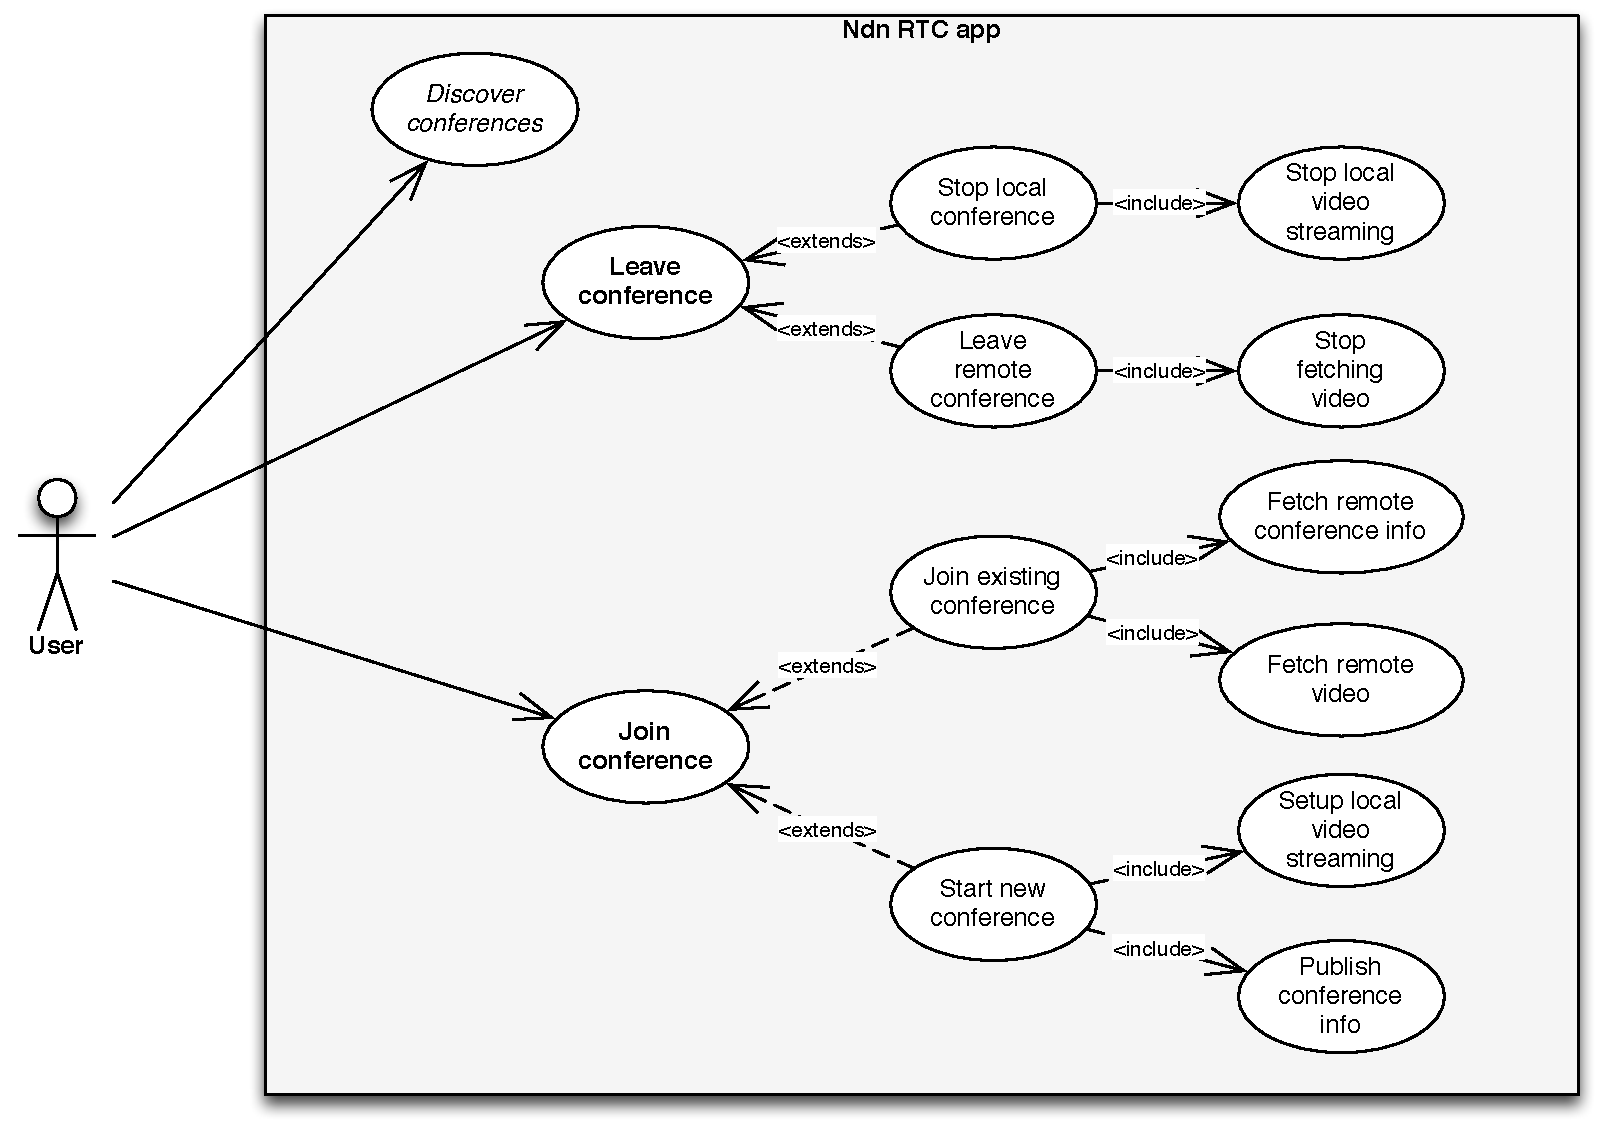
\includegraphics[width=\textwidth]{../res/graphics/addon-uc}
\caption{Add-on Use-Cases}
\label{fig:uc}
\end{figure}

Top-view architecture of the add-on is presented on Figure \ref{fig:arch}.
\begin{figure}
\centering
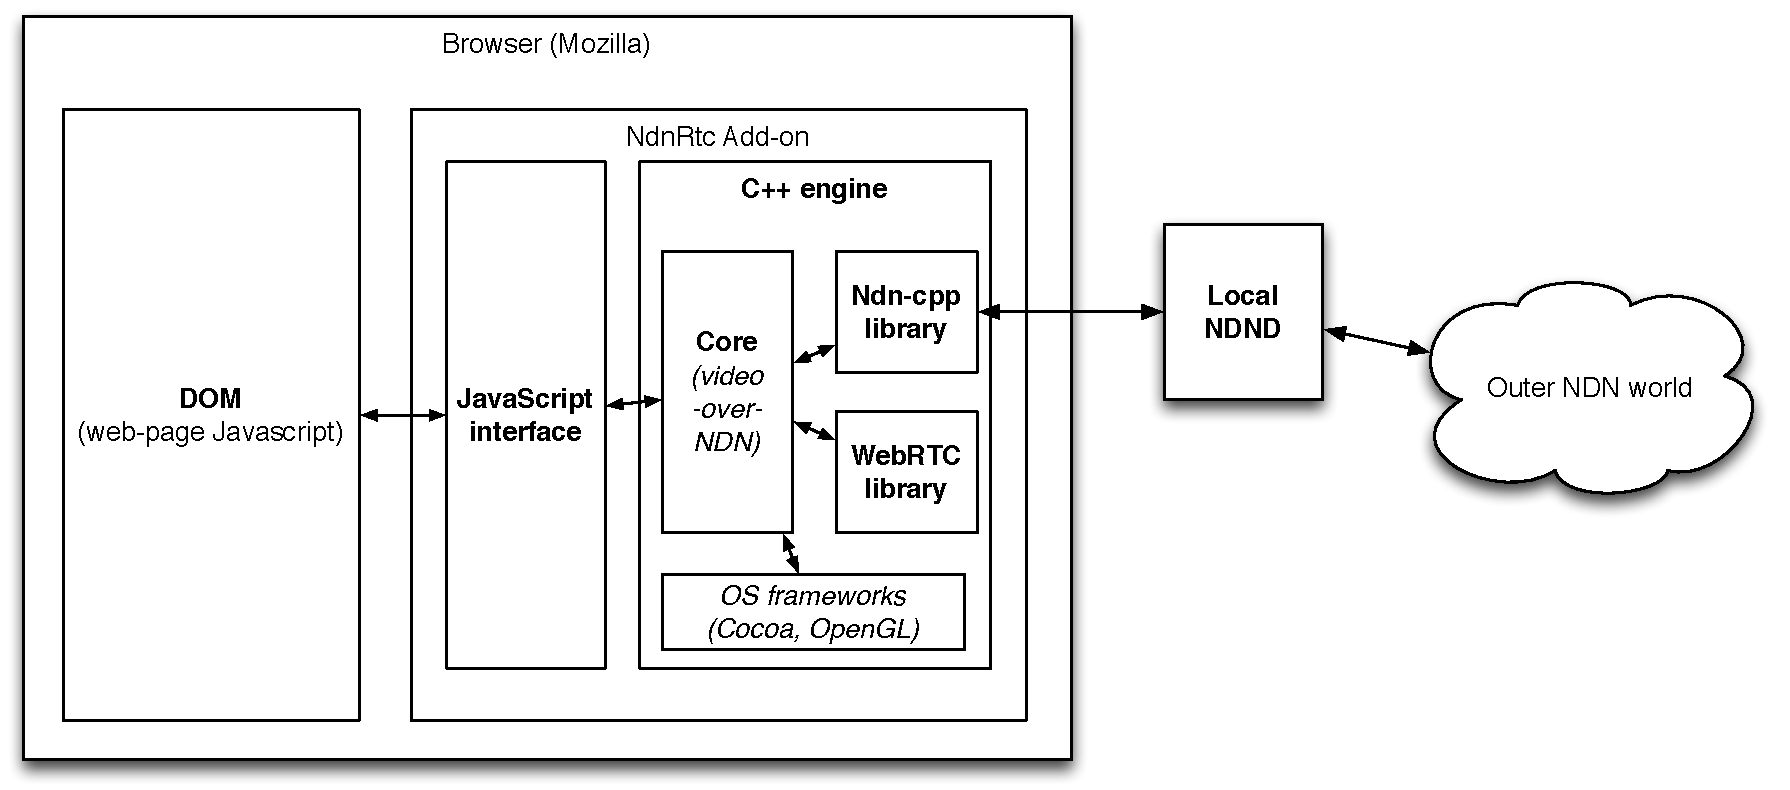
\includegraphics[width=\textwidth]{../res/graphics/addon-arch}
\caption{Add-on architecture}
\label{fig:arch}
\end{figure}

\subsection{C++ Firefox add-on}
This sections describes the internal architectural approach for the C++ part of the add-on.

One can start learning how the add-on works by looking at the sequence diagrams of the main use-cases: Starting a conference (Figure \ref{fig:start}), Joining an existing conference (Figure \ref{fig:join}) and Leaving a conference (Figure \ref{fig:leave}).

\begin{figure}
\centering
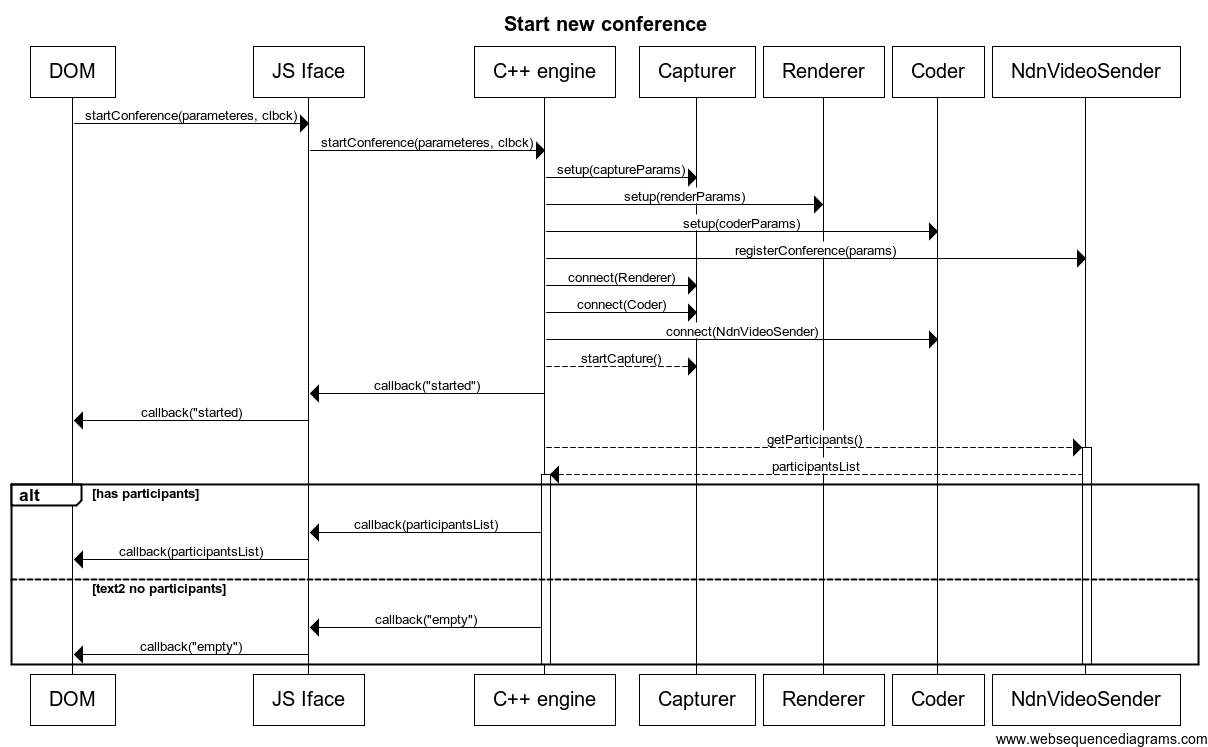
\includegraphics[width=\textwidth]{../res/graphics/start-seq}
\caption{Sequence diagram for starting a conference}
\label{fig:start}
\end{figure}

\begin{figure}
\centering
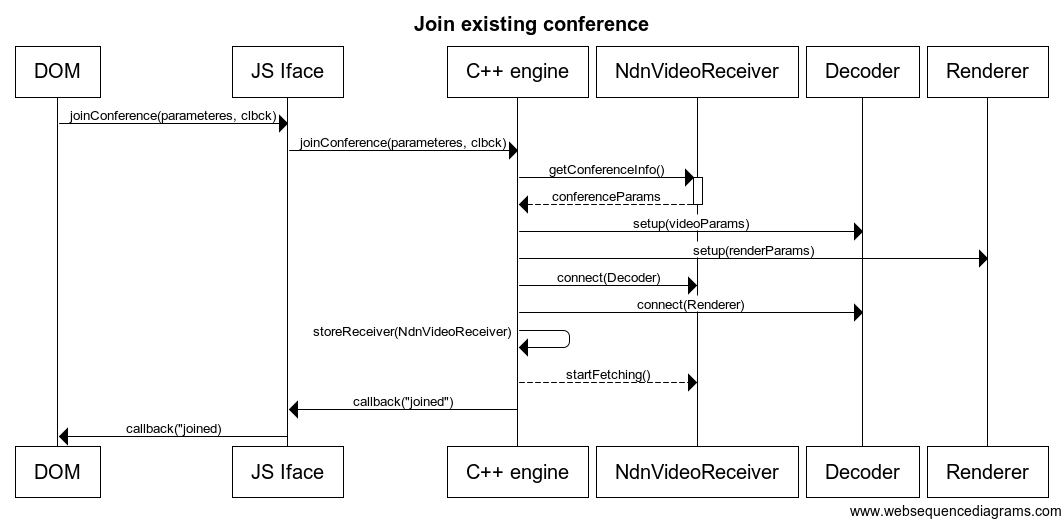
\includegraphics[width=\textwidth]{../res/graphics/join-seq}
\caption{Sequence diagram for joining an existing conference}
\label{fig:join}
\end{figure}

\begin{figure}
\centering
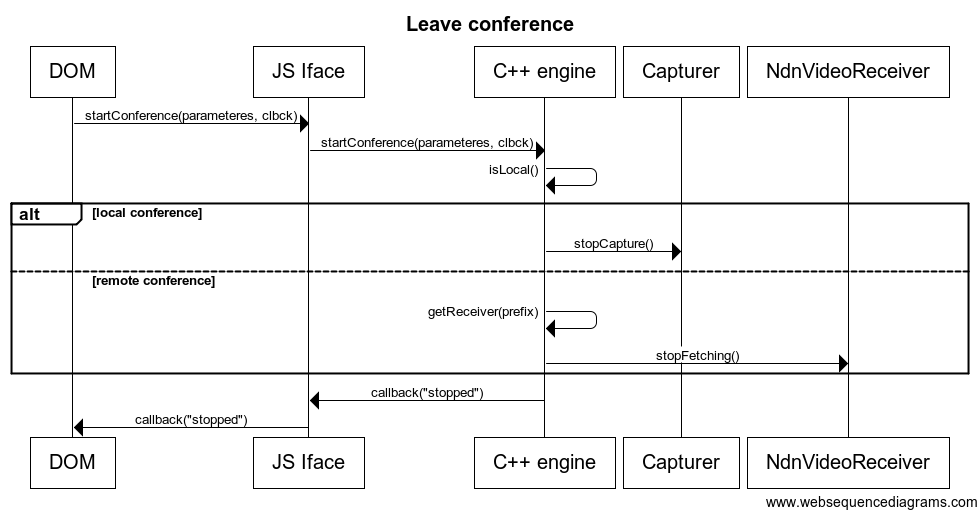
\includegraphics[width=\textwidth]{../res/graphics/leave-seq}
\caption{Sequence diagram for leaving a conference}
\label{fig:leave}
\end{figure}


\subsection{Javascript Web application}
\subsubsection{Overview}
\subsubsection{UI design}

\section{Next steps}
\begin{itemize}
\item Provide user authentication in video conferences
\item Implement secure media transfer
\item Scalable video encoding
\end{itemize}

\section{References} \cite{videoTR}, \cite{ChronosTR}
%************************************************
\bibliography{../res/bib/ndn-np}
\bibliographystyle{plain}



\end{document}